\section{The Data}
\label{sec:data}

{\bf
We used the Kepler-Gaia cross-matched catalog that is available at
https://gaia-kepler.fun.
This catalog contains \nfun\ Kepler targets, cross-matched with Gaia targets
within in a 1'' radius and includes positions, parallaxes, and proper motions
from Gaia EDR3 and RVs from Gaia DR2.
}
We crossmatched this catalog with the catalog of photogeometric
distances inferred from Gaia EDR3 parallaxes \citep{bailer-jones2021} and
applied corrections to EDR3 parallaxes based on \citet{lindegren2021b}.
% created using the cross-match service and Vizier catalogue access tool
% provided by CDS, Strasbourg, France, as well as the astroquery and astropy
% python packages.
We also crossmatched this catalog with the LAMOST DR5 catalog and the APOGEE
DR16 stellar catalog \citep{cui2012, apogee_dr16, xiang2019}.
We removed stars with angular separations larger than 150 milliarcseconds
during each of these crossmatches.
Stars with effective temperatures that differed by more than 500K between
Gaia, APOGEE, and LAMOST were removed from the sample to minimize incorrect
crossmatches.
To remove stars with multiple crossmatches within 150 milliarcseconds, we only
kept the star with the smallest angular separation.
We also removed stars with a Gaia parallax $<$ 0, parallax signal-to-noise
ratio $<$ 10, and Gaia astrometric excess noise $>$ 5.
To preferentially select single stars, we removed stars with {\tt ruwe} $\geq$
1.4, {\tt ipd\_frac\_multi\_peak} $>2$, and {\tt
ipd\_gof\_harmonic\_amplitude} $\geq$ 0.1.
APOGEE reports VSCATTER, which is the error-deconvolved scatter in the
individual time-series RV measurements for each source and can indicate that a
star is a binary.
We removed 208 stars in our final sample with APOGEE VSCATTER greater than 1
\kms.
After applying these cuts our total number of targets was \nstars.
In total, \nrv\ stars in our sample have at least one RV measurement from
Gaia, LAMOST, or APOGEE; \ngaia\ have RVs from Gaia DR2, \nlamost\ from LAMOST
DR5, and \napogee\ from APOGEE DR16.
The APOGEE survey \citep[R $=$ 22,500;][]{apogee} has a higher spectral
resolution than Gaia \citep[R $=$ 11,500;][]{cropper2018}, which in turn is
higher than LAMOST \citep[R $=$ 1,800;][]{zhao2012}.
The median RV uncertainty for stars in our sample is around 0.1 km/s for
APOGEE RVs, 1 km/s for Gaia RVS, and 5 km/s for
LAMOST RVs.
In cases where stars had two or more available RV measurements, we adopted
APOGEE RVs as a first priority, followed by Gaia, then LAMOST.

Although RVs are available for more than one in three Kepler targets, most
stars with RV measurements are bright.
Very few of the faintest stars have RVs because of the selection functions of
spectroscopic surveys.
% In our sample, one in 2.5 stars hotter than 5000 K had RV measurements,
% whereas only one in six stars cooler than 5000 K had RVs.
Most of the stars in our sample with Gaia RV measurements are brighter than
around 14th magnitude in Gaia $G$-band, and stars with LAMOST or APOGEE RVs
are mostly brighter than around 16th magnitude.
Figure \ref{fig:rv_histogram} shows the apparent magnitude distributions of
the stars in our sample, with and without RVs.
This figure reveals the combined selection functions of the Gaia, LAMOST and
APOGEE RV surveys and shows that faint stars are less likely to have RV
measurements than bright ones.
\begin{figure}[ht!]
\caption{
    % The apparent magnitude (left) and temperature (right) distributions of
    % stars in our sample, with and without RV measurements from \gaia\ and
    % \lamost.
    The distribution of apparent Gaia magnitudes for
    stars in our sample with and without RV measurements from Gaia, LAMOST and
    APOGEE.
}
  \centering 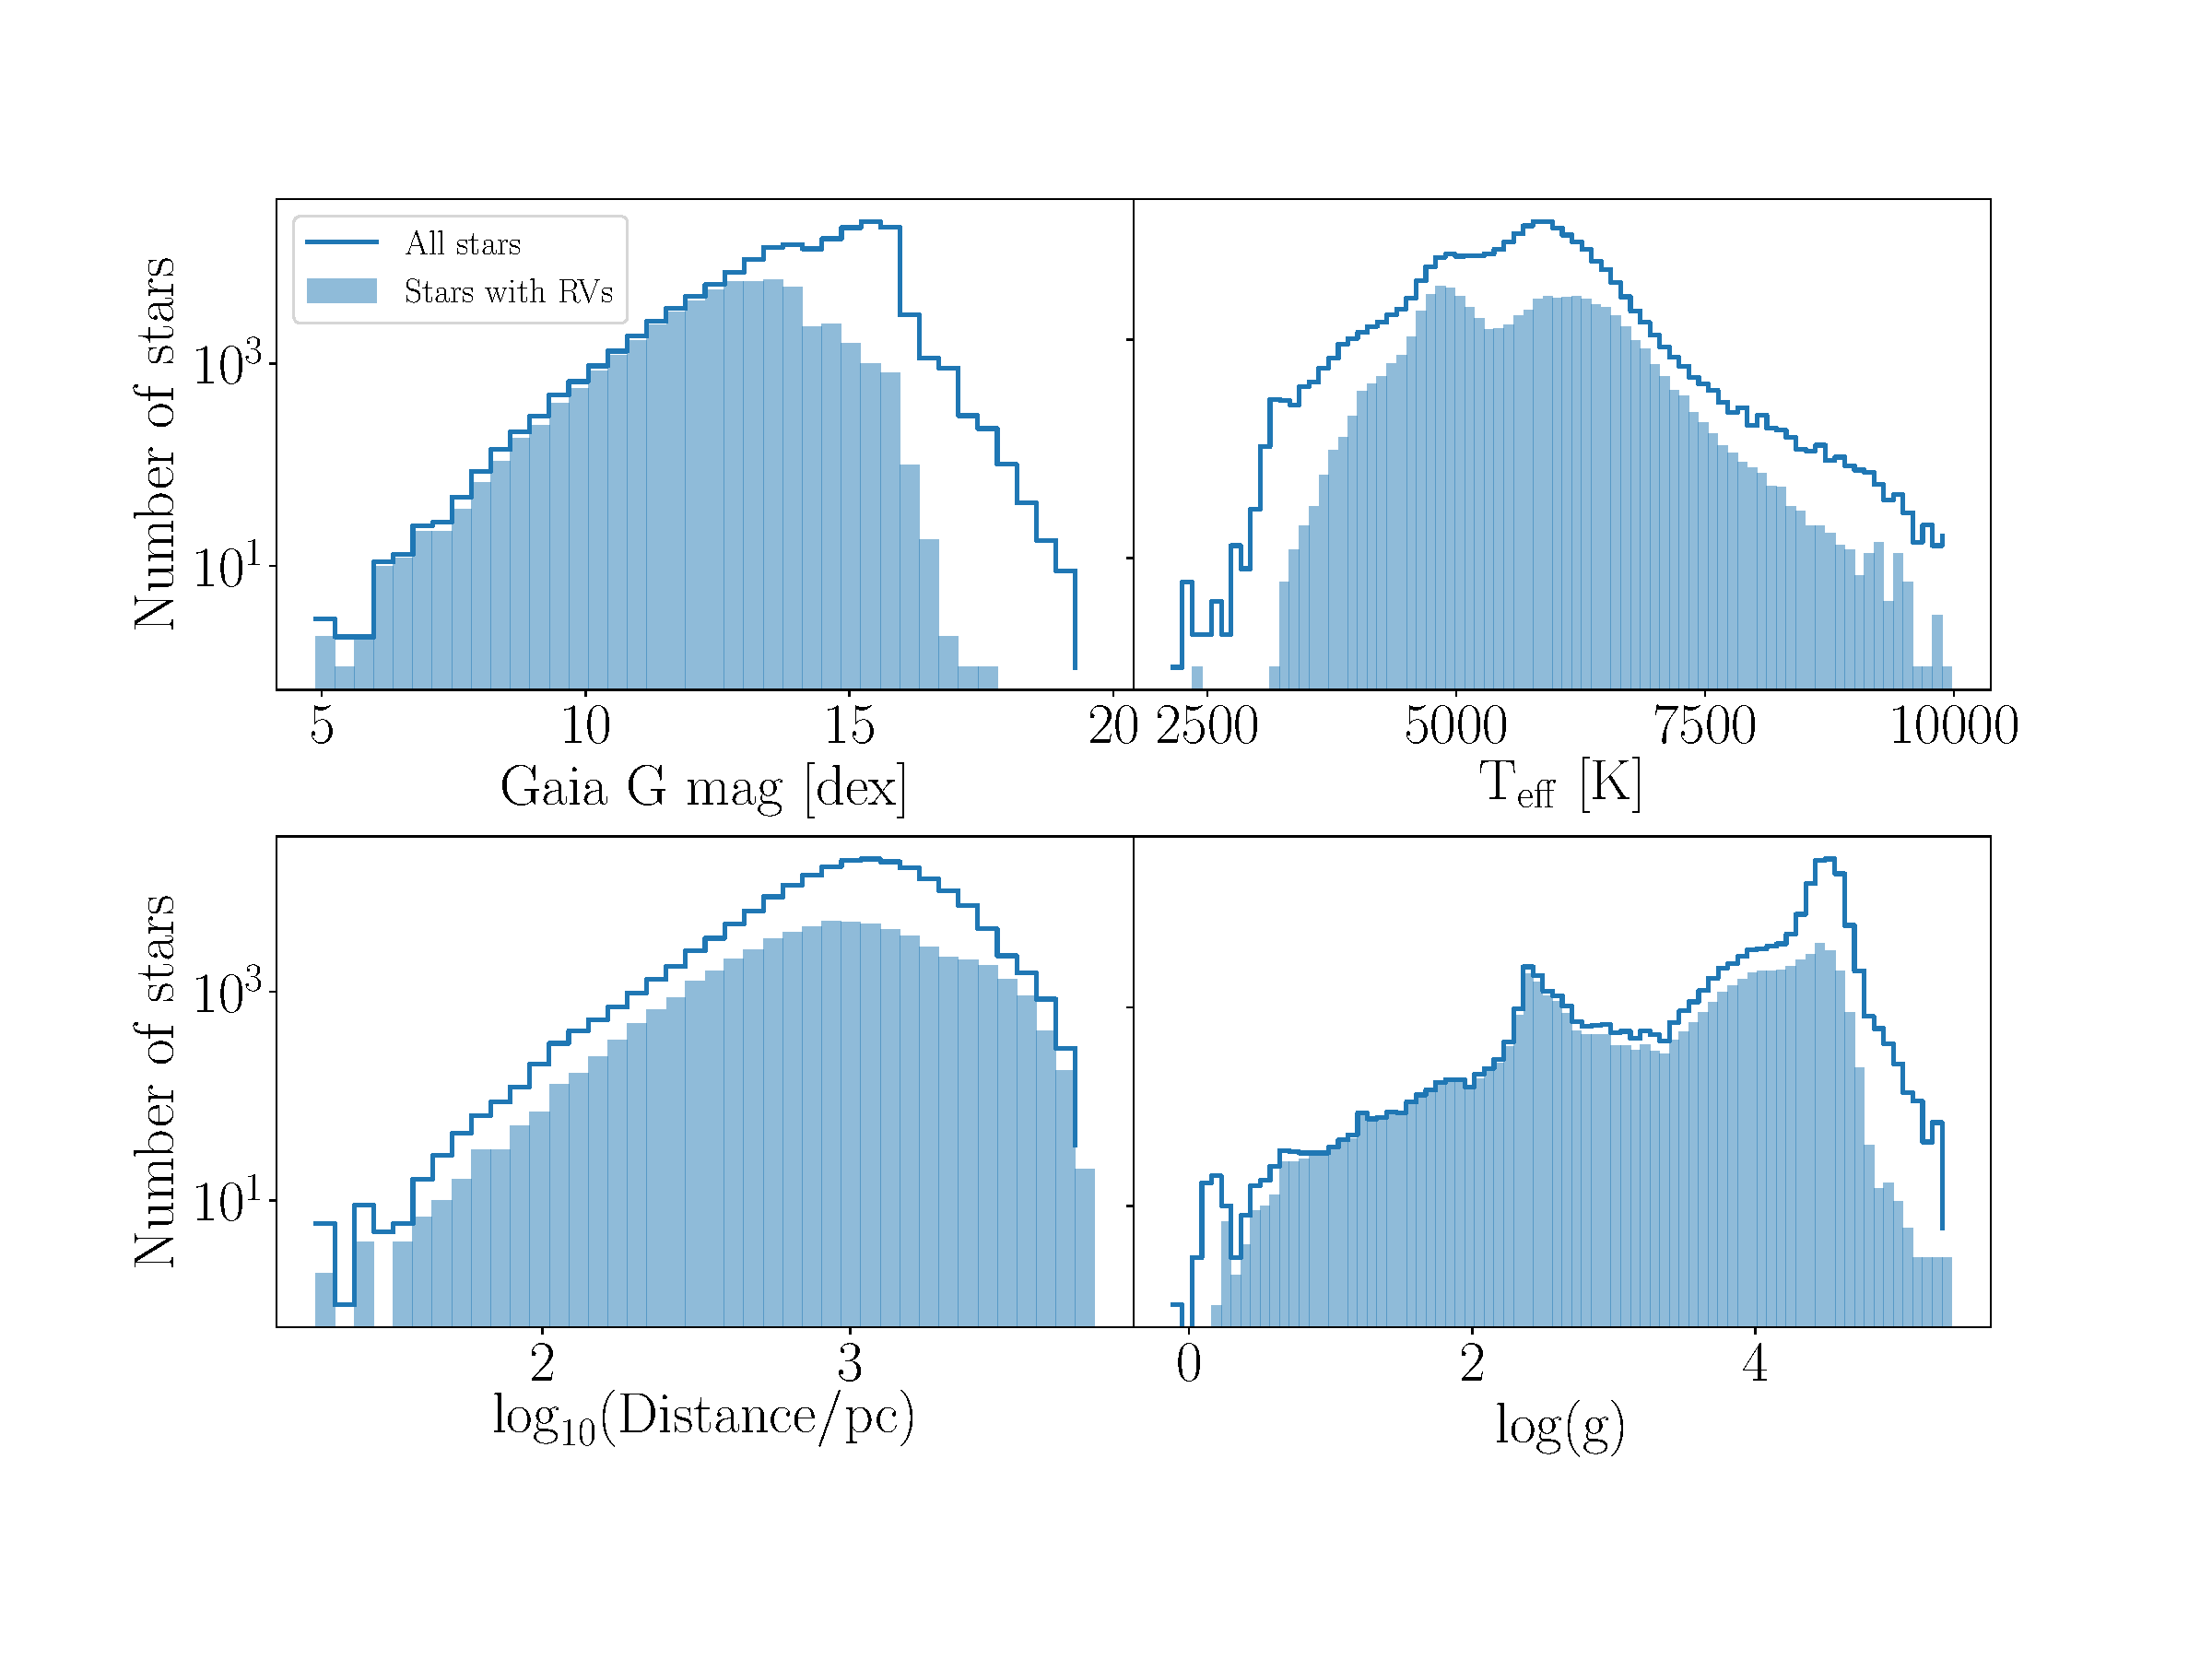
\includegraphics[width=.5\textwidth]{rv_histogram}
\label{fig:rv_histogram}
\end{figure}

To illustrate how the populations of stars with and without RVs differ, we
plot them on a color-magnitude diagram (CMD) in figure \ref{fig:CMD}.
The stars with RVs are generally hotter and more luminous than stars without.
Most stars with RVs fall on the upper main sequence, the red giant branch, and
the red clump.
Most stars without RVs fall on the main sequence.
This overall selection function is a combination of the APOGEE, LAMOST and
Gaia DR2 selection functions.

In this paper, we construct a prior using stars with RV measurements which we
then use to infer the velocities of stars without RV measurements.
However, given that the populations of stars with and without RVs are so
different, this could bias the velocities we infer, particularly if they are
prior-dependent.
We investigate this idea in section \ref{sec:prior} and find that the \vx\ and
\vz\ velocities we infer are relatively insensitive to the prior and therefore
unlikely to biased, however the \vy\ velocities we infer should be used with
caution as they are relatively prior-dependent.
\begin{figure}[ht!]
\caption{
    A magnitude-temperature diagram of stars in the Kepler field with (left)
    and without (right) RVs provided by Gaia, LAMOST and APOGEE.
    The stars with RVs are generally hotter and more luminous than those
    without RVs, and include a large number of red clump stars and red giant
    branch stars.
    Stars without RVs are mostly concentrated on the main sequence.
}
  \centering 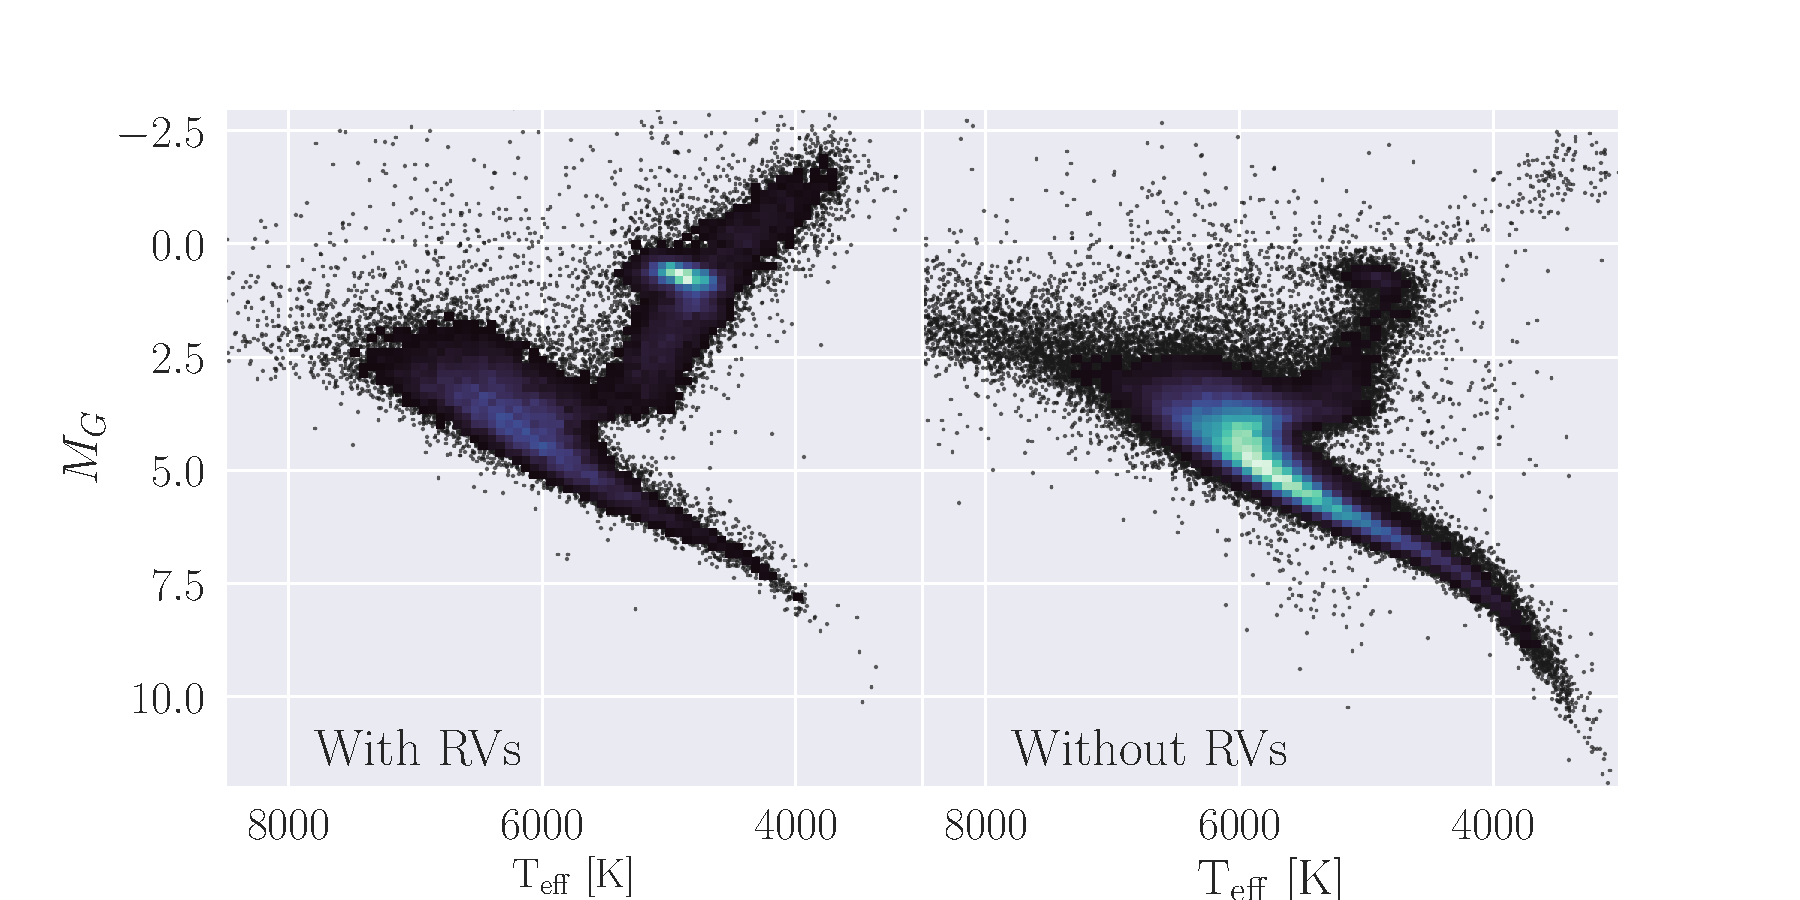
\includegraphics[width=1\textwidth]{CMD}
\label{fig:CMD}
\end{figure}
